\documentclass{prova}

\usepackage{amssymb}
\usepackage{gensymb}

\renewcommand{\sin}{\mbox{sen}}
\newcommand{\ra}{\rightarrow}
\newcommand{\lra}{\leftrightarrow}
\newcommand{\Ra}{\Rightarrow}
\newcommand{\LRa}{\Leftrightarrow}
\renewcommand{\lnot}{\sim}
\newcommand{\larg}{\vdash}

\professor{Prof. Adriano Barbosa}
\disciplina{Introdução ao Cálculo}
\avaliacao{P2}
\curso{Matem\'atica}
\data{18/09/2020}

\begin{document}
    \cabecalho{6}  % o numero 5 indica a qnt de quadros na tabela de nota
    
    \textbf{Todas as respostas devem ser justificadas.}
    \begin{questionario}
	\q{Uma escala de temperatura misteriosa $M$ está relacionada com a
	   escala Celsius de modo que as temperaturas de $42\degree C$ e
	   $13\degree C$ são equivalentes a $0\degree M$ e $100\degree M$,
	   respectivamente. Determine a temperatura na escala $M$ em que a
	   água congela.}
	\q{Uma sequência com $2020$ hexágonos foi montada como na figura abaixo.
	   Quantas arestas existem na sequência?}
	   \begin{figure}[h]
               \centering
	       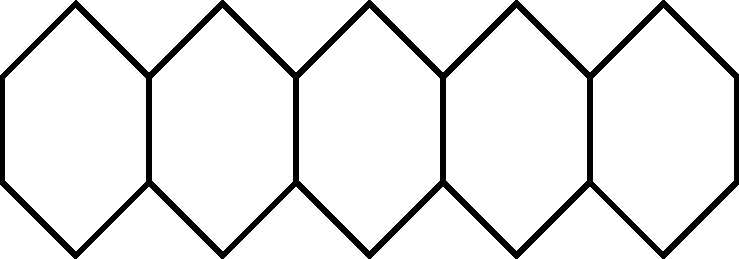
\includegraphics[width=0.4\textwidth]{fig1.pdf}
	   \end{figure}
	\q{A capacidade de transporte de uma caminhonete é de 30 sacos de
	   cimento ou 200 telhas. Se a caminhonete já está carregada com 11
	   sacos de cimento, quantas telhas (inteiras) ainda podem ser
	   carregadas no máximo?}
	\q{Encontre a função quadrática cujo gráfico é dado na figura abaixo:}
	   \begin{figure}[h]
	       \centering
	       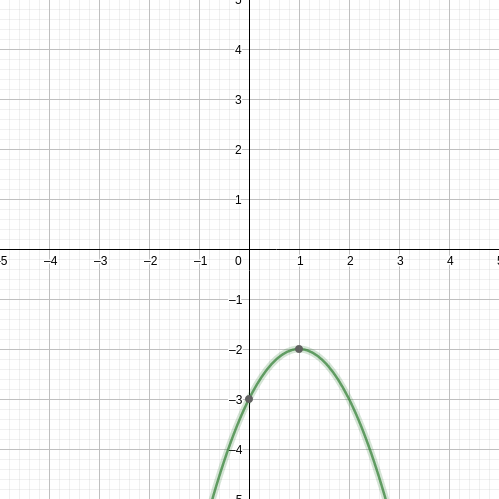
\includegraphics[width=0.4\textwidth]{fig2.png}
           \end{figure}
	\newpage{}
	\q{Deseja-se cercar a maior área retangular possível junto a um rio com
	   $40$ metros de cerca. Encontre as medidas dos lados do retângulo e
	   a área da região cercada.}
	   \begin{figure}[h]
	       \centering
	       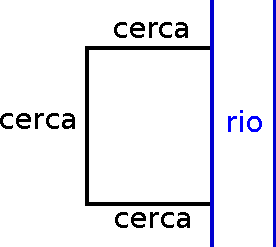
\includegraphics[width=0.3\textwidth]{fig3.pdf}
           \end{figure}
	\q{Uma sorveteria vende $130$ picolés por dia por R\$ $5,00$ cada.
	   Observou-se que, durante uma promoção de verão, cada vez que
	   diminuia R\$ $0,50$ no preço do picolé, vendia $20$ unidades a mais
	   por dia. Qual deve ser o preço do picolé para que a receita da
	   sorveteria seja máxima?}
    \end{questionario}
\end{document}
